\section{Literature Review}
\subsection{ DPSN (Deep Photometric Stereo Network)}

\begin{figure}[h]

\centering
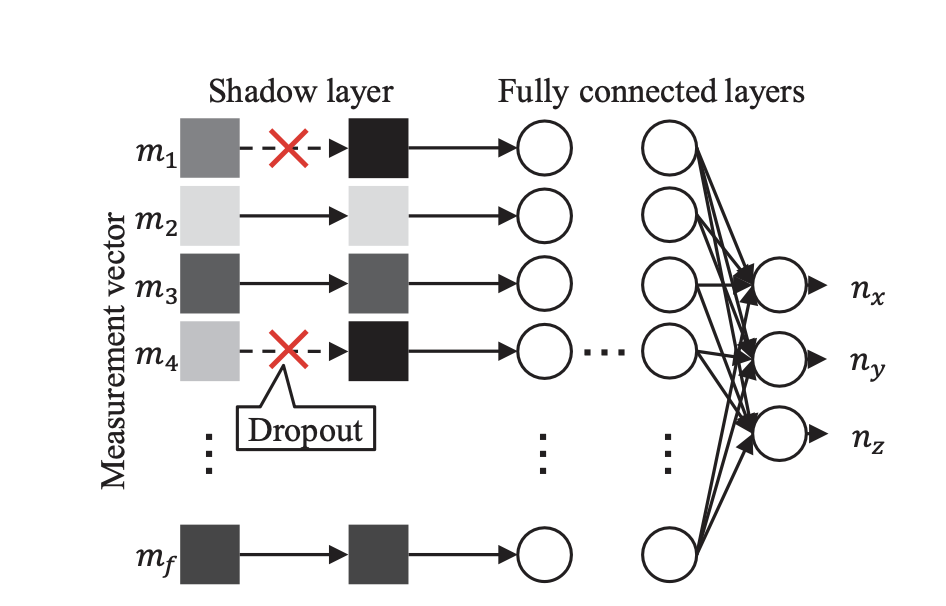
\includegraphics[scale=0.5]{figures/dpsn.png}
\caption{Overview of the proposed network. It consists of two components, the shadow layer and fully connected layers. In the shadow layer, some of the measurement vector elements are ran- domly dropped to simulate the cast shadow effect. In this figure, $m_1$ and $m_4$ are dropped and corresponding values of the input vector are set to 0.
}
\label{fig:dpsn}
\end{figure}

The proposed Differentiable Per-Pixel Surface Normal (DPSN)\cite{dpsn} network is a multi-layer neural network that learns a mapping from a measurement vector $\mathbf{m} \in \mathbb{R}^f$ obtained under $f$ different light directions to the surface normal $\mathbf{n} \in \mathbb{R}^3$. The DPSN operates in a per-pixel manner for both training and prediction. We assume that the light directions $\mathbf{L} = [\mathbf{l}_1, \ldots, \mathbf{l}_f] \in \mathbb{R}^{3 \times f}$ are known and consistent between the training and prediction phases. Our method utilizes simulated observations generated from diverse surface normals rendered using the MERL BRDF\cite{merl} database, which contains BRDFs of 100 different real-world materials.

Next, we describe the structure of the proposed network, as well as its key features and some limitations.
\subsubsection{Network architecture}

The core of DPSN is a deep neural network with fully connected layers (see Fig.\ref{fig:dpsn}). It takes a measurement vector as input, where each element represents the light intensity observed from a specific light direction. The network then outputs the predicted surface normal for that pixel location. Before feeding the measurement vector to the network, it's normalized to have a unit length. Notably, the network processes each color channel from the measurement vector independently.

A significant challenge in photometric stereo is cast shadow, which can't be modeled accurately by standard methods. To address this, DPSN incorporates a "shadow layer" inspired by the dropout technique. Dropout randomly removes units during training to prevent overfitting. Similarly, the shadow layer randomly sets some elements of the input vector to zero, simulating pixels in shadow regions. By training with this shadow layer, the network learns to handle diverse materials and cast shadows effectively.

Unlike conventional dropout that scales the output, the shadow layer directly sets shadowed elements to zero. The dropout rate (r) controls the proportion of pixels simulated to be in shadow. Since the actual shadow distribution is usually unknown, the training process uses a range of dropout rates to make the network robust.

The DPSN architecture is summarized in table (\ref{tab:dpsn_layers}). It consists of seven layers: a shadow layer followed by six dense layers. Each dense layer uses ReLU activation and dropout during training. The network is trained by minimizing a loss function that compares the predicted surface normal with the ground truth value. The Adam optimizer with default settings is used for optimization.

\begin{table}[ht]
    \centering
    \begin{tabular}{|c|l|}
        \hline
        \textbf{Layer} & \textbf{Composition} \\
        \hline
        1 & Shadow Layer \\
        2 & Dense-(4096), ReLU, Dropout \\
        3 & Dense-(4096), ReLU, Dropout \\
        4 & Dense-(2048), ReLU, Dropout \\
        5 & Dense-(2048), ReLU, Dropout \\
        6 & Dense-(2048), ReLU, Dropout \\
        7 & Dense-(3) \\
        \hline
    \end{tabular}
    \caption{Neural network layers in the proposed DPSN.}
    \label{tab:dpsn_layers}
\end{table}

\subsubsection{Key features}
Learn a flexible mapping between complex reflectance observations and surface normals: Unlike traditional methods relying on simplified reflectance models (e.g., Lambert's model), DPSN utilizes a deep neural network to capture intricate relationships between real-world lighting conditions and surface normals. This allows it to handle complex reflectance behavior beyond the limitations of pre-defined models.


\subsubsection{Limitations}

One limitation of their method is the requirement for predefined and consistent light directions during both training and testing. This is because their training relies on simulated observations generated under specific lighting conditions. Ideally, the photometric stereo data should be captured with a fixed lighting setup (camera and light sources) to avoid retraining for each lighting scenario. 

The proposed method's reliance on a relatively simple neural network architecture could potentially limit its accuracy, especially when dealing with complex surface geometries and challenging lighting conditions. While the fully connected layers provide a straightforward approach for learning the mapping between measurement vectors and surface normals, more sophisticated network architectures, such as convolutional neural networks (CNNs) or recurrent neural networks (RNNs), might be able to capture more intricate spatial relationships and temporal dependencies in the data, potentially leading to improved accuracy.

\subsection{PS-FCN (Photometric Stereo - Fully Convolutional Network)}
A deep fully convolutional network\cite{ps-fcn}, called PS-FCN, that takes an arbitrary number of images of a static object captured under different light directions with a fixed camera as input, and predicts a normal map of the object in a fast feed-forward pass. Unlike the prior proposed learning based method, PS-FCN does not require a pre-defined set of light directions during training and testing, and can handle multiple images and light directions in an order-agnostic manner. Although PS-FCN was trained on synthetic data, it can generalize well on real datasets. 

It was showed that PS-FCN can be easily extended to handle the problem of uncalibrated photometric stereo by combining with LC-Net. Note that in this case, PS-FCN is exactly the same as NE-Net.



\subsubsection{Network Architecture}

\begin{figure}[h]

\centering
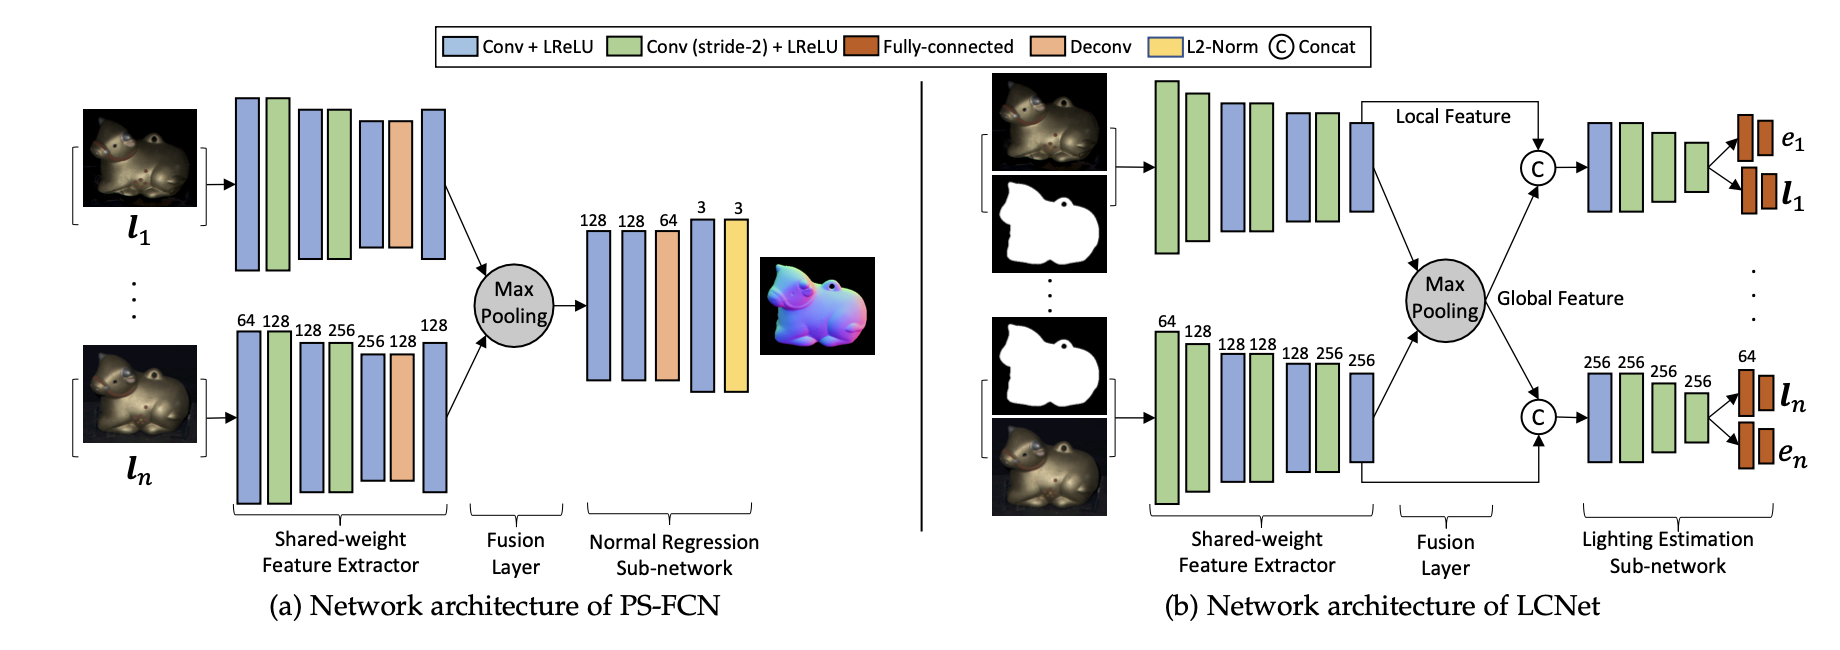
\includegraphics[scale=0.5]{figures/psfcn.png}
\caption{Overview of the proposed method. Values above the layers indicate the number of feature channels.
}
\label{fig:ps-fcn}
\end{figure}

PS-FCN is a multi-branch siamese network consisting of three components: a shared-weight feature extractor, a fusion layer, and a normal regression network (see Fig.\ref{fig:ps-fcn}). It can be trained and tested using an arbitrary number of images with their associated light directions as input.

For an object captured under $q$ distinct light directions, we repeat each light direction (i.e., a 3-vector) to form a 3-channel image having the same spatial dimension as the input image ($3 \times h \times w$), and concatenate it with the input image. Hence, the input to our model has a dimension of $q \times 6 \times h \times w$. We separately feed the image-light pairs to the shared-weight feature extractor to extract a feature map from each of the inputs, and apply a max-pooling operation in the fusion layer to aggregate these feature maps. Finally, the normal regression network takes the fused feature map as input and estimates a normal map of the object.

The shared-weight feature extractor has seven convolutional layers, where the feature map is down-sampled twice and then up-sampled once, resulting in a down-sample factor of two. This design can increase the receptive field and preserve spatial information with a small memory consumption. The normal regression network has four convolutional layers and up-samples the fused feature map to the same spatial dimension as the input images. An L2-normalization layer is appended at the end of the normal regression network to produce the normal map.

PS-FCN is a fully convolutional network, and it can be applied to datasets with different image scales. Thanks to the max-pooling operation in the fusion layer, it possesses the order-agnostic property. Besides, PS-FCN can be easily extended to handle uncalibrated photometric stereo, where the light directions are not known, by simply removing the light directions during training.

\subsubsection{Loss Function}

The learning of our PS-FCN is supervised by the estimation error between the predicted and the ground-truth normal maps. We formulate our loss function using the commonly used cosine similarity loss:

\[
L_{\text{normal}} = \frac{1}{hw} \sum_{i,j} (1 - N_{ij} \cdot \tilde{N}_{ij})
\]

where $N_{ij}$ and $\tilde{N}_{ij}$ denote the predicted normal and the ground truth, respectively, at the point $(i, j)$. If the predicted normal has a similar orientation as the ground truth, the dot-product $N_{ij} \cdot \tilde{N}_{ij}$ will be close to 1, and the loss will be small; vice versa. Other losses like mean square error can also be adopted.

\subsubsection{Key features}
PS-FCN accepts an arbitrary number of images and their associated light directions as input and regresses an accurate normal map. PS-FCN does not require a pre-defined set of light directions during training and testing, and allows the light directions used in testing different from that used in training. It can handle multiple images and light directions in an order-agnostic manner. In order to train PS-FCN, two synthetic datasets with various realistic shapes and materials have been created. After training, PS-FCN can generalize well on challenging real datasets. In addition, PS-FCN can be easily extended to handle uncalibrated photometric stereo. Results on diverse real datasets have clearly shown that PS-FCN outperforms previous calibrated photometric stereo methods, and promising results have been achieved in uncalibrated scenario.
\subsubsection{Limitations}
Overfitting: Like any CNN-based model, PS-FCN might be susceptible to overfitting, especially if the training dataset for surface normals and corresponding images is limited. Overfitting occurs when the model learns the specifics of the training data too well and performs poorly on unseen data.

Limited Generalizability to Complex Materials: CNNs excel at learning patterns from data, but their performance can be hindered when encountering materials with complex reflectance properties not well represented in the training dataset. PS-FCN might struggle with surfaces exhibiting strong non-Lambertian reflectance behavior (where light reflection is not uniform across all angles).

Computational Cost: While potentially more efficient than fully connected networks, processing high-resolution images with CNNs can still be computationally expensive. This could limit PS-FCN's applicability to real-time applications or scenarios with resource constraints.

Limited Understanding of Underlying Physics:  CNNs are often considered black boxes, meaning their internal decision-making processes are not easily interpretable. This could be a limitation if understanding the physical aspects of surface normal estimation is crucial for the application.

Sensitivity to Noise: CNNs can be sensitive to noise present in the images used for training and prediction. This noise could lead to inaccurate surface normal estimations by PS-FCN.

\subsection{SDPS (Self-calibrating Deep Photometric Stereo Networks)}

This paper proposes an uncalibrated photometric stereo method for non-Lambertian scenes based on deep learning\cite{sdps}. Unlike previous approaches that heavily rely on assumptions of specific reflectances and light source distributions, our method is able to determine both shape and light directions of a scene with unknown arbitrary reflectances observed under unknown varying light directions. To achieve this goal, the author group proposed a two-stage deep learning architecture, called SDPS-Net, which can effectively take advantage of intermediate supervision, resulting in reduced learning difficulty compared to a single-stage model. Experiments on both synthetic and real datasets show that the proposed approach significantly outperforms previous uncalibrated photometric stereo methods.


\subsubsection{Discretization of Lighting Space}

Since we cast our lighting estimation as a classification problem, we need to discretize the continuous lighting space. A light direction in the upper hemisphere can be described by its azimuth $\phi \in [0^\circ, 180^\circ]$ and elevation $\theta \in [-90^\circ, 90^\circ]$ (see Fig.\ref{fig:discretization}(a)). To discretize the light direction space, we evenly divide both the azimuth and elevation into $K_d$ bins, resulting in $K_d^2$ classes (see Fig.\ref{fig:discretization}(b)). Solving a $K_d^2$-class classification problem is computationally inefficient, as the softmax probability vector will have a very high dimension even when $K_d$ is not large (e.g., $K_d^2 = 1,296$ when $K_d = 36$). Instead, we estimate the azimuth and elevation of a light direction separately, leading to two $K_d$-class classification problems. Similarly, we evenly divide the range of possible light intensities into $K_e$ classes (e.g., $K_e = 20$ for a possible light intensity range of $[0.2, 2.0]$).

\begin{figure}[h]

\centering
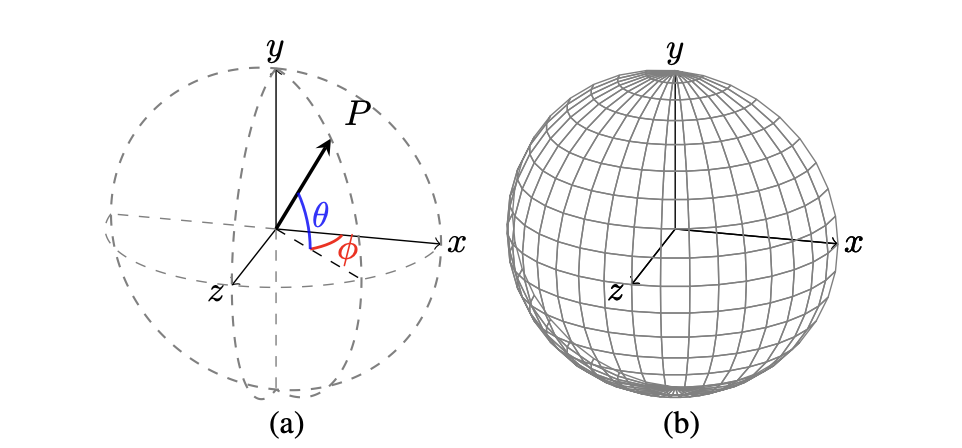
\includegraphics[scale=0.5]{figures/discretization.png}
\caption{(a) Illustration of the coordinate system (z axis is the viewing direction). $\phi \in [0^\circ, 180^\circ]$ and $\theta \in [-90^\circ, 90^\circ]$ are the azimuth and elevation of the light direction, respectively. (b) Ex-
ample discretization of the light direction space when $K_d = 18$.
}
\label{fig:discretization}
\end{figure}

\subsubsection{Local-Global Feature Fusion}

A straightforward approach to estimate the lighting for each image is simply taking a single image as input, encoding it into a feature map using a CNN, and feeding the feature map to a lighting prediction layer. However, the result of such a simple solution is far from satisfactory. The appearance of an object is determined by its surface geometry, reflectance model, and the lighting. The feature map extracted from a single observation obviously does not provide sufficient information for resolving the shape-light ambiguity.

Thanks to the nature of photometric stereo, where multiple observations of an object are considered, we propose a local-global feature fusion strategy to extract more comprehensive information from multiple observations. Specifically, we separately feed each image into a shared-weight feature extractor to extract a feature map, which we call the local feature as it only provides information from a single observation. All local features of the input images are then aggregated into a global feature through a max-pooling operation, which has been proven to be efficient and robust in aggregating salient features from a varying number of unordered inputs [33, 5]. This global feature is expected to convey implicit surface geometry and reflectance information of the object, helping to resolve the ambiguity in lighting estimation.

Each local feature is concatenated with the global feature and fed to a shared-weight lighting estimation sub-network to predict the lighting for each individual image. By considering both local and global features, our model can produce much more reliable results than using the local features alone. Additionally, empirically including the object mask as input can effectively improve the performance of lighting estimation, as will be seen in the experiment section.
\subsubsection{Network Architecture: LCNet}

\begin{figure}[h]

\centering
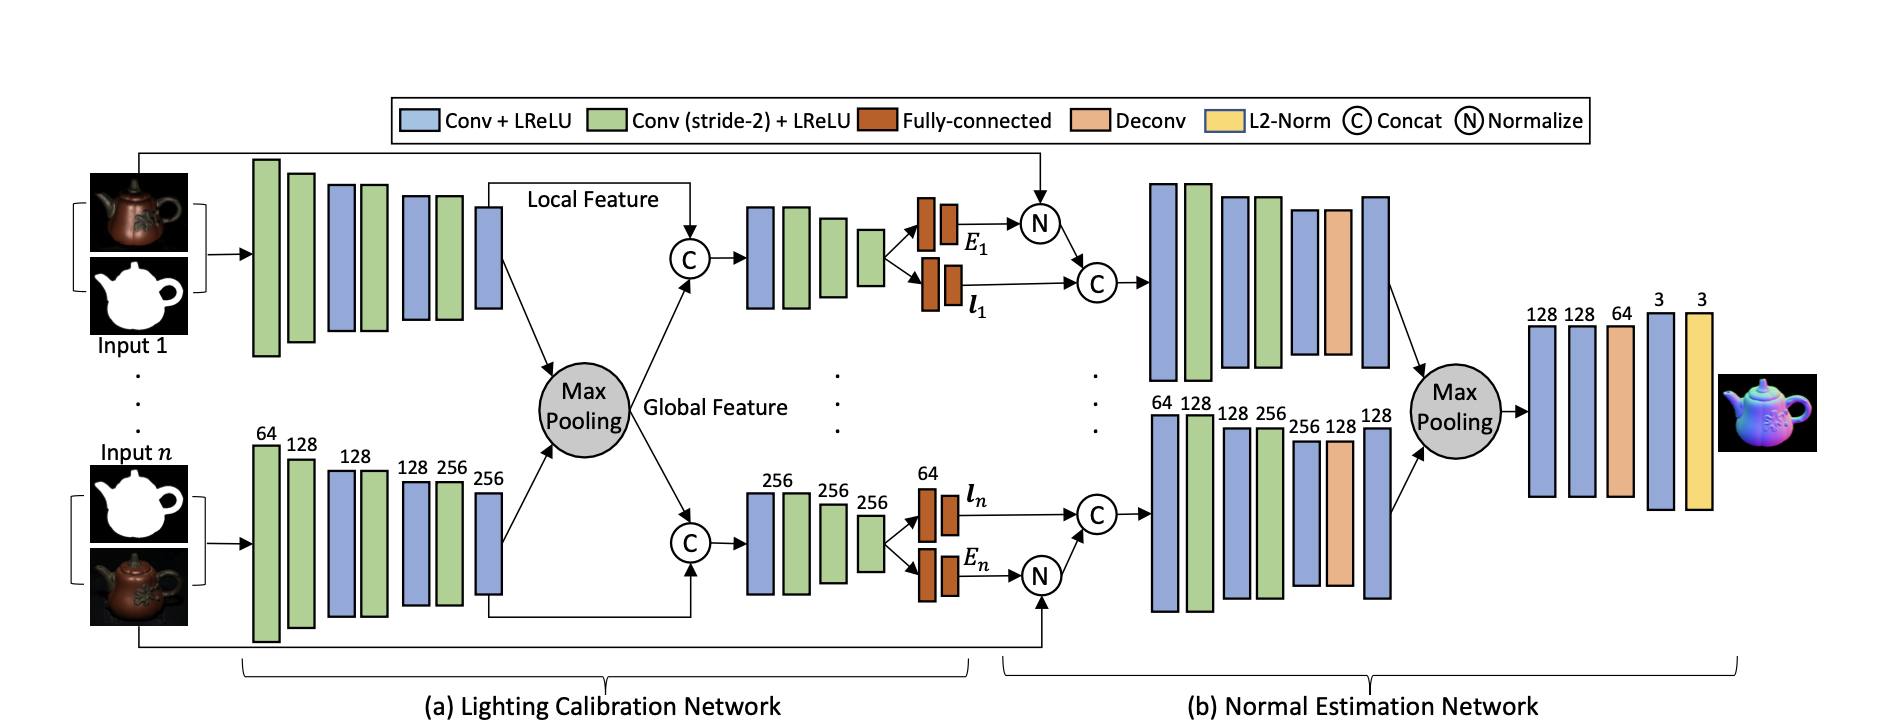
\includegraphics[scale=0.5]{figures/sdps.png}
\caption{The network architecture of SDPS-Net is composed of (a) Lighting Calibration Network and (b) Normal Estimation Network. Kernel sizes for all convolutional layers are $3 \times 3$, and values above the layers indicate the number of feature channels.
}
\label{fig:sdps}
\end{figure}

LCNet is a multi-input-multi-output (MIMO) network that consists of a shared-weight feature extractor, an aggregation layer (i.e., max-pooling layer), and a shared-weight lighting estimation sub-network (see Fig.\ref{fig:sdps}(a)). It takes the observations of the object together with the object mask as input and outputs the light directions and intensities in the form of softmax probability vectors of dimension $K_d$ (azimuth), $K_d$ (elevation), and $K_e$ (intensity), respectively. We convert the output of LCNet to 3-vector light directions and scalar intensity values by simply taking the middle value of the range with the highest probability.

\subsubsection{Loss Function for Lighting Estimation}

Multi-class cross-entropy loss is adopted for both light direction and intensity estimation. The overall loss function is defined as:

\[ L_{\text{Light}} = \lambda_{la} L_{la} + \lambda_{le} L_{le} + \lambda_e L_e \]

where $L_{la}$ and $L_{le}$ are the loss terms for azimuth and elevation of the light direction, and $L_e$ is the loss term for light intensity. During training, weights $\lambda_{la}$, $\lambda_{le}$, and $\lambda_e$ for the loss terms are set to 1.

\subsubsection{Normal Estimation Network: NENet}

NENet is a multi-input-single-output (MISO) network. Its architecture is similar to PS-FCN [5], consisting of a shared-weight feature extractor, an aggregation layer, and a normal regression sub-network (see Fig.\ref{fig:sdps}(b)). The key difference between NENet and PS-FCN is that PS-FCN requires accurate lightings as input, whereas NENet is trained with discretized lightings estimated by LCNet and shows a more robust behavior over noise in the lightings.

NENet first normalizes the input images using the light intensities predicted by LCNet and then concatenates the light directions predicted by LCNet with the images to form the input of the shared-weight feature extractor. Given an image of size $h \times w$, the loss function for NENet is defined as:

\[ L_{\text{Normal}} = \frac{1}{hw} \sum_{i} (1 - n_i^\top n_{\tilde{i}}) \]

where $n_i$ and $n_{\tilde{i}}$ denote the predicted normal and the ground truth, respectively, at pixel $i$.


\subsubsection{Key Features}

\begin{enumerate}
    \item \textbf{Multi-Input-Multi-Output (MIMO) Architecture (LCNet):}
    \begin{itemize}
        \item LCNet incorporates multiple observations of the object along with an object mask as input.
        \item Outputs light directions and intensities using softmax probability vectors.
        \item Provides flexibility in handling different lighting conditions.
    \end{itemize}
    
    \item \textbf{Discretization of Lighting Space:}
    \begin{itemize}
        \item Efficiently handles the classification problem by separately estimating azimuth and elevation.
        \item Divides the range of possible light intensities into discrete classes.
    \end{itemize}
    
    \item \textbf{Local-Global Feature Fusion:}
    \begin{itemize}
        \item Aggregates local features from individual observations into a global feature using max-pooling.
        \item Helps resolve shape-light ambiguity by considering both local and global information.
    \end{itemize}
    
    \item \textbf{Robust Behavior with Noise in Lightings (NENet):}
    \begin{itemize}
        \item Normal Estimation Network (NENet) is trained with discretized lightings estimated by LCNet.
        \item Shows robustness to noise in the lightings.
    \end{itemize}
\end{enumerate}

\subsubsection{Limitations}

\begin{enumerate}
    \item \textbf{Computationally Intensive:}
    \begin{itemize}
        \item The softmax probability vectors for a large number of classes can be computationally expensive.
        \item Discretization of lighting space may lead to increased complexity.
    \end{itemize}
    
    \item \textbf{Dependency on Accurate Lightings:}
    \begin{itemize}
        \item LCNet relies on accurate lightings as input.
        \item Errors in lighting estimation can propagate to subsequent stages.
    \end{itemize}
    
    \item \textbf{Shape-Light Ambiguity:}
    \begin{itemize}
        \item Despite local-global fusion, resolving shape-light ambiguity remains challenging.
        \item Single observations may not provide sufficient information.
    \end{itemize}
    
    \item \textbf{Uncalibrated Photometric Stereo:}
    \begin{itemize}
        \item While LCNet can handle uncalibrated photometric stereo, it requires removing light directions during training.
        \item Handling unknown light directions remains an open challenge.
    \end{itemize}
\end{enumerate}


\subsection{SDM-UniPS} 
The challenging universal photometric stereo task, recently introduced in \cite{unips}, makes no assumptions about surface geometry, material properties, or lighting conditions. The objective of this task is to recover a normal map $\mathbf{N} \in \mathbb{R}^{H \times W \times 3}$ from images $\mathbf{I}_k \in \mathbb{R}^{H \times W \times 3}; k \in \{1, \ldots, K\}$ captured under $K$ unknown lighting conditions using an orthographic camera. Optionally, an object mask $\mathbf{M} \in \mathbb{R}^{H \times W}$ may be provided.

The proposed method, SDM-UniPS \cite{sdm}, is illustrated in Figure~\ref{fig:sdm}. Given pre-processed images and an optional object mask, feature maps for each lighting condition are extracted through interactions along the spatial and light axes (i.e., the scale-invariant spatial-light feature encoder). Randomly sampled locations from the coordinate system of the input image are then used for bilinearly interpolating features at these locations.

Features and raw observations at each location are aggregated pixel-wise, and surface normals are recovered from the aggregated features after non-local spatial interaction among them (i.e., the pixel-sampling Transformer). In line with \cite{unips}, the focus is on describing high-level concepts rather than providing detailed explanations for the sake of clarity. Refer to the appendix for a comprehensive description of the network architectures.

\begin{figure}[h]

\centering
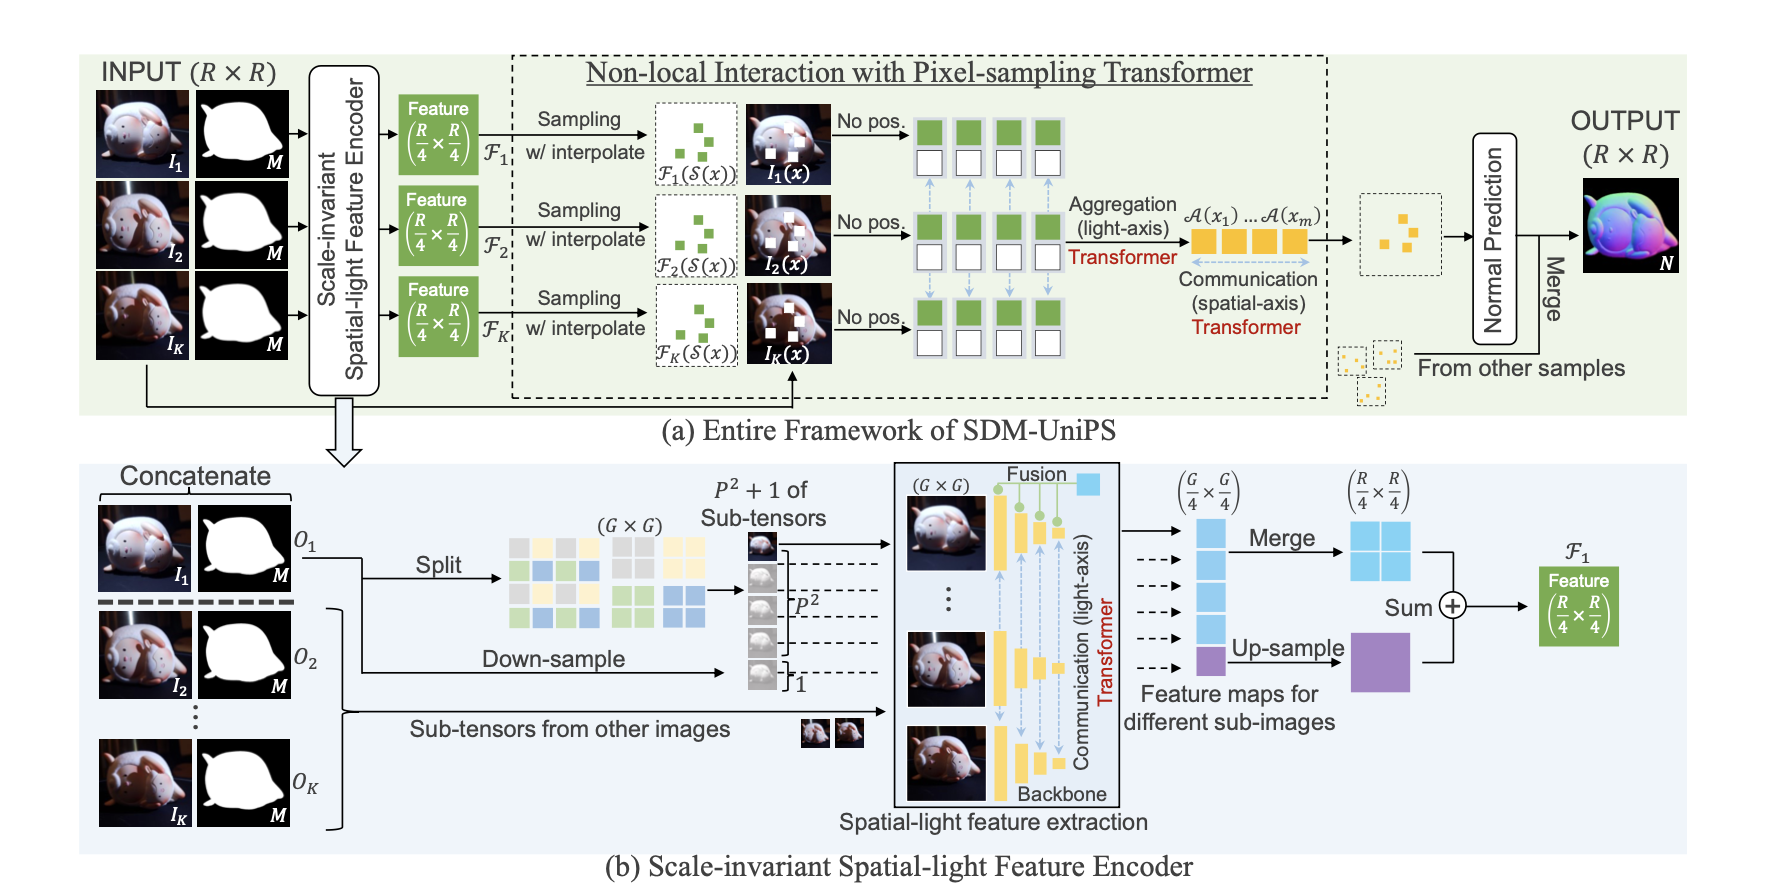
\includegraphics[scale=0.5]{figures/sdm.png}
\caption{The entire framework is illustrated in (a). Given multiple images and an object mask (optional), the scale-invariant spatial-light encoder (detailed in (b)) extracts a feature map for each image. The surface normal vectors are independently recovered at each of pixel samples (i.e., 2048) after the non-local interaction among aggregated features from interpolated feature maps and raw observations.
}
\label{fig:sdm}
\end{figure}

\subsubsection{Key Features}

\textbf{Pre-processing:} Input images are resized or cropped to a resolution ($R$) that is divisible by 32, which is compatible with most hierarchical vision backbones. To ensure similar image value ranges, each image is normalized by a random value between its maximum and mean.

\textbf{Scale-invariant Spatial-light Feature Encoder:} After pre-processing, feature maps from images and an optional object mask are extracted through interactions along both spatial and light axes. Following the basic framework in \cite{unips}, each image and object mask\footnote{Without a mask, a matrix with all values set to one is concatenated.} are concatenated to form a tensor $\mathbf{O}_k \in \mathbb{R}^{R \times R \times 4}$, which is then input to the common vision backbone to extract hierarchical feature maps $\mathbf{B}_k \in \mathbb{R}^{S_s \times S_s \times C_s}; s \in \{1, 2, 3, 4\}$. Here, $S_s \in \{4, 8, 16, 32\}$ represents the scale of the $s$-th feature map, and $C_s$ is the dimension of features at that scale. For each feature scale, features from different tensors at the same pixel interact with each other along the light-axis using naïve Transformers . Finally, hierarchical feature maps are fused to $\mathbf{F}_k \in \mathbb{R}^{R/4 \times R/4 \times C_F}$ using the feature pyramid network, where $C_F$ is the output feature dimension. Unlike \cite{unips}, a varying number of Transformer blocks are used at each hierarchy scale (i.e., the number of blocks changes from $[1, 1, 1, 1]$ to $[0, 1, 2, 4]$) so that the deeper features interact more than the shallow ones.

\textbf{Non-local Interaction with Pixel-sampling Transformer:} Given the scale-invariant spatial-light feature maps $\mathbf{F}_k$ and images $\mathbf{I}_k$, surface normals are recovered after pixel-wise feature aggregation along the light-axis (i.e., the light channel shrinks from $K$ to 1). Feature aggregation under different lighting conditions is fundamental in photometric stereo networks, with various strategies studied, such as observation maps, max-pooling, graph-convolution, and self-attention. The Transformer model with self-attention is utilized as in the encoder following UniPS \cite{unips}. 

UniPS directly predicts surface normals from pixel-wise aggregated feature vectors, following other pixel-wise methods, without considering non-local interactions. However, aggregated features lose lighting-specific information, obtaining lighting-invariant representations more related to surface attributes. Considering non-local interactions of aggregated features at multiple surface points is crucial in physics-based tasks.

Applying image-wise neural networks like CNNs on the aggregated feature map demands enormous computational cost for large output resolutions (e.g., $2048 \times 2048$) and risks compromising output normal map details. To address these issues, inspiration is drawn from recent Transformers on 3-D points, applying a Transformer on a fixed number ($m$) of pixel samples (e.g., $m = 2048$) from random locations in the input coordinate system. This is termed the pixel-sampling Transformer. Unlike image-based approaches, the pixel-sampling Transformer's memory consumption is constant per sample set, scaling to arbitrary image sizes. Moreover, by applying the Transformer to a randomly sampled set of locations, local interactions that may lead to over-smoothing of feature maps (e.g., in CNNs) are almost entirely eliminated.

Concretely, given $m$ random pixels $x_i=1, \ldots, m$ from the masked region of the input coordinate system, features are interpolated at those pixels as $\mathbf{F}_{1,\ldots,K}(\mathcal{S}(x_i))$, where $\mathcal{S}$ is the bilinear interpolation operator. Then, interpolated features are concatenated with corresponding raw observations $\mathbf{I}_{1,\ldots,K}(x_i)$ and aggregated to $\mathcal{A}(x_i)$ with pooling by multi-head attention (PMA). Given aggregated features at different pixels in the same sample set, another naïve Transformer is applied to perform non-local interactions. Since the goal of this process is to consider surface-level interactions based on physical attributes, pixel coordinate information is unnecessary. Thus, position embeddings are not applied to samples, unlike most existing visual Transformer models, allowing the samples to propagate their aggregated features without location information.

After the non-local interaction, a two-layer MLP is applied to predict surface normals at sampled locations. Finally, surface normals for each set are merged to obtain the final surface normal map at the input image resolution. This pixel-sampling Transformer approach facilitates non-local interactions while maintaining computational efficiency and preserving output normal map details, making it suitable for physics-based tasks with high-resolution images.

\subsubsection{Network Architecture Details}

The entire framework consists of six sub-networks. The scale-invariant spatial-light encoder includes (a) a backbone network for image-wise feature extraction, (b) a Transformer network for pixel-wise interaction along the light-axis, and (c) a feature pyramid network for the fusion of hierarchical feature maps. In the pixel-sampling Transformer, there are (d) a Transformer network for feature aggregation along the light-axis and (e) a Transformer network for feature interaction along the spatial-axis. Finally, there is (f) an MLP for surface normal prediction. Each network architecture is detailed below.

\textbf{Backbone:} In the scale-invariant spatial-light encoder, each sub-tensor (i.e., concatenation of a sub-image and a sub-mask) is independently input to ConvNeXt, a modernized ResNet-like architecture inspired by the recent Vision Transformer. The variants of ConvNeXt differ in the number of channels $C$ and the number of ConvNeXt blocks $B$ in each stage. The following configuration is used:
\begin{itemize}
    \item ConvNeXt-T: $C = (96, 192, 384, 768)$, $B = (3, 3, 9, 3)$
\end{itemize}
The ConvNeXt block includes 7x7 depthwise convolution, 1x1 convolution with the inverted bottleneck design (4x hidden dimension), and 1x1 convolution to undo the hidden dimension. Between convolutions, layer normalization and GeLU activation are applied. The output of ConvNeXt is a stack of feature maps of $(B \times 96 \times R/4 \times R/4)$, $(B \times 192 \times R/8 \times R/8)$, $(B \times 384 \times R/16 \times R/16)$, and $(B \times 768 \times R/32 \times R/32)$ where $B$ is the batch size and $R$ is the input sub-tensor size.

\textbf{Transformer (interaction along light-axis):} Given hierarchical feature maps from the backbone network, a Transformer is applied pixel-wise to features of individual scales along the light-axis. The number of channels in a hidden layer $C$ and the number of Transformer blocks $B$ are as follows:
\begin{itemize}
    \item Transformer: $C = (96, 192, 384, 768)$, $B = (0, 1, 2, 4)$
\end{itemize}
The Transformer block projects the input feature to query, key, and value vectors with dimensions identical to the input. These are then passed to a multi-head self-attention (with 8 heads) followed by a softmax and a feed-forward network with two linear layers, where the inner layer's dimensionality is twice that of the input. Each of the two sub-layers is followed by layer normalization and dropout ($p = 0.1$).

\textbf{Feature pyramid network:} After the hierarchical feature maps interact pixel-wise using Transformers, feature maps of different scales corresponding to each input image are fused with the feature pyramid network (i.e., UPerNet). The output feature size is $(B \times R/4 \times R/4 \times 256)$.

\textbf{Transformer (aggregation along light-axis):} Given $m$ pixel locations at the input coordinate system, each pair of a raw observation and a bilinearly interpolated feature vector from the output of the feature pyramid network is concatenated to a vector of dimension 259 (i.e., 256+3). The feature aggregation network takes $K$ sets of 259-dimensional feature vectors at the same location as input and performs two Transformer blocks of $C=256$ (shrunk from 259 to 256 by QKV projection). The output feature is further concatenated with the raw observation, and each 259-dimensional feature vector is again fed to another three Transformer blocks of $C=256$. The output $K$ feature vectors are then passed to PMA, where the number of elements in a set is shrunk from $K$ to one using another Transformer block of $C=384$.

\textbf{Transformer (interaction along spatial-axis):} At the final step of the pixel-sampling Transformer module, two Transformer blocks ($C=384$) are used to communicate features among the $m$ locations. Naïve self-attention requires $O(m^2)$ memory consumption; however, $m$ (i.e., the number of pixel samples) is much larger than $K$ (i.e., the number of input images), making increasing sample size difficult. Therefore, the $O(m)$ implementation of self-attention is used to tackle this problem.

\textbf{Normal prediction network:} The surface normal predictor is an MLP with one hidden layer, where the feature dimension shrinks from 384 to 192 to 3, and the norm of the output vector is normalized to be a unit surface normal vector at the location.

\subsubsection{Limitations}
Firstly, although the proposed method works robustly for versatile lighting conditions, it is not very effective when the lighting variations are minimal. In scenarios with limited lighting variation, the model struggles to accurately capture the necessary details for precise normal map recovery. This limitation arises because the model relies on significant differences in lighting to discern the surface details and depth variations. When the lighting is too uniform, the essential cues for distinguishing these features become insufficient, leading to suboptimal performance.

Secondly, the proposed method can easily be extended beyond normal map recovery by replacing the loss and data. In reality, attempts to output Bidirectional Reflectance Distribution Function (BRDF) parameters for materials have been made. However, due to fundamental ambiguities, it is difficult to evaluate the recovered BRDF parameters. These ambiguities stem from the inherent complexity and variability of material properties, which make it challenging to unambiguously determine the BRDF parameters from photometric data alone. The BRDF encapsulates how light reflects off a surface, and minor changes in surface properties can lead to significant variations in the reflected light. Consequently, the recovered BRDF parameters may not accurately represent the true material properties, complicating the evaluation process.

Additionally, the extension to BRDF parameter recovery introduces further complexities. The BRDF space is high-dimensional, and accurately mapping photometric data to this space requires comprehensive datasets and sophisticated models. Even slight errors in the input data or model assumptions can lead to substantial deviations in the recovered parameters. This sensitivity to input conditions highlights the need for more robust algorithms and extensive datasets to improve the accuracy of BRDF recovery.
